\section{\gds{} Validation}
\label{sec:gds-validation}

The \gds{} framework introduced in \Cref{sec:gds} is designed to measure
how much a team \emph{deserved} to win, independently of the stochastic
outcomes -- turnover bounces, blocked kicks, last-second field goals -- that
ultimately determine the scoreboard. Before the archetype analysis of
\Cref{sec:archetype-findings}, it is necessary to demonstrate that \gds{}
scores are meaningfully related to competitive outcomes: a framework that
correlates poorly with wins at both the game and season level would have
limited utility as a basis for strategic classification. This section presents
four complementary validation analyses. First, game-level winner prediction
accuracy is compared against a na\"{i}ve baseline. Second, the season-level
correlation between \gds{}/game and win percentage is quantified and
decomposed. Third, the component structure of the top and bottom teams in the
2024 NFL season is examined to demonstrate the diversity of winning formulas
the framework captures. Fourth, a luck analysis identifies teams whose actual
win totals diverged substantially from their \gds{}-implied expectations,
quantifying the role of variance in converting deserved performance into
observed outcomes.

%  -- -- -- -- -- -- -- -- -- -- -- -- -- -- -- -- -- -- -- --
\subsection{Game-Winner Prediction Accuracy}
\label{sec:game-winner-prediction}

The most direct validation of a game-quality metric is its ability to identify
which team played better in the sense of subsequently winning the game.
Concretely, the question is: when a team finishes a game with a higher \gds{}
than its opponent, does that team win more often than not? An affirmative answer
would confirm that \gds{} tracks the underlying competitive process rather than
capturing statistical noise.

Across the 1{,}848 regular-season games contested from 2018 to 2024 (excluding
7 ties), the team with the higher \gds{} won 1{,}592 times, corresponding to a
game-winner prediction accuracy of \textbf{86.1\%}. This result is particularly notable
because the comparison is noiseless in the sense relevant here: the \gds{} of
each team is computed entirely from their own offensive execution on that
specific game day, without any use of the final score or of the opponent's
identity as a contextual input. The framework is answering the question ``which
team generated and suppressed scoring-probability more effectively?'' and the
answer corresponds to the actual winner in more than four of every five games.

The appropriate baseline for comparison is not a random 50\% coin flip, since
NFL games are not symmetric: home teams win approximately 57\% of regular-season
games across the study window, reflecting the well-documented home-field
advantage in professional American football \parencite{lopez2018randomness}. The
\gds{} accuracy of 86.1\% is substantially above this baseline, representing an
improvement of 29.1 percentage points over the home-team heuristic.

The 13.9\% of games where the higher-\gds{} team loses represents a substantive
finding rather than a model failure. These divergences are precisely the games
where football's structural variance -- turnover outcomes, field goal efficiency,
explosive-play variance in a small-sample game -- decouples the underlying
performance process from the scoreboard. From the perspective of the \gds{}
framework, these are games where the ``wrong'' team won in the probabilistic
sense. Their existence confirms that the metric is not simply a re-encoding of
the final score, but captures an orthogonal dimension of performance quality
that the final score only imperfectly reflects. This property -- that \gds{}
measures who \emph{deserved} to win rather than who \emph{did} win -- is the
foundational motivation for its use in archetype classification.

%  -- -- -- -- -- -- -- -- -- -- -- -- -- -- -- -- -- -- -- --
\subsection{Season-Level Correlation with Win Percentage}
\label{sec:season-correlation}

Game-level accuracy confirms that \gds{} tracks the better team within a single
contest. The season-level analysis asks whether teams that accumulate high
average \gds{} scores across a full season also win more games, which is the
relevant question for strategic evaluation. The unit of analysis is the
team-season: 32 teams across seven seasons from 2018 to 2024 yield $n = 224$
observations.

The Pearson correlation between mean \gds{}/game and season win percentage is
$r = 0.858$ ($p = 3.24 \times 10^{-66}$), with a coefficient of determination
$R^2 = 0.736$. The interpretation is direct: \gds{}/game accounts for
\textbf{73.6\%} of the variance in team win percentage across all team-seasons
in the study window. The correlation is highly statistically significant by
any conventional threshold, with the $p$-value functionally indistinguishable
from zero at any reasonable significance level \parencite{yurko2019nflwar}.

This result establishes the framework's claim to construct validity: a metric
that is intended to measure team-level competitive quality should correlate
strongly with competitive outcomes, and $R^2 = 0.736$ confirms that it does
(\Cref{fig:gds-winpct}). The remaining 26.4\% of win-percentage variance is
attributable to factors that a performance-based metric cannot capture,
including within-game variance in turnover outcomes, opponent strength effects
not absorbed into the \gds{} framework, and genuine randomness in close-game
resolutions.

\begin{figure}[htbp]
  \centering
  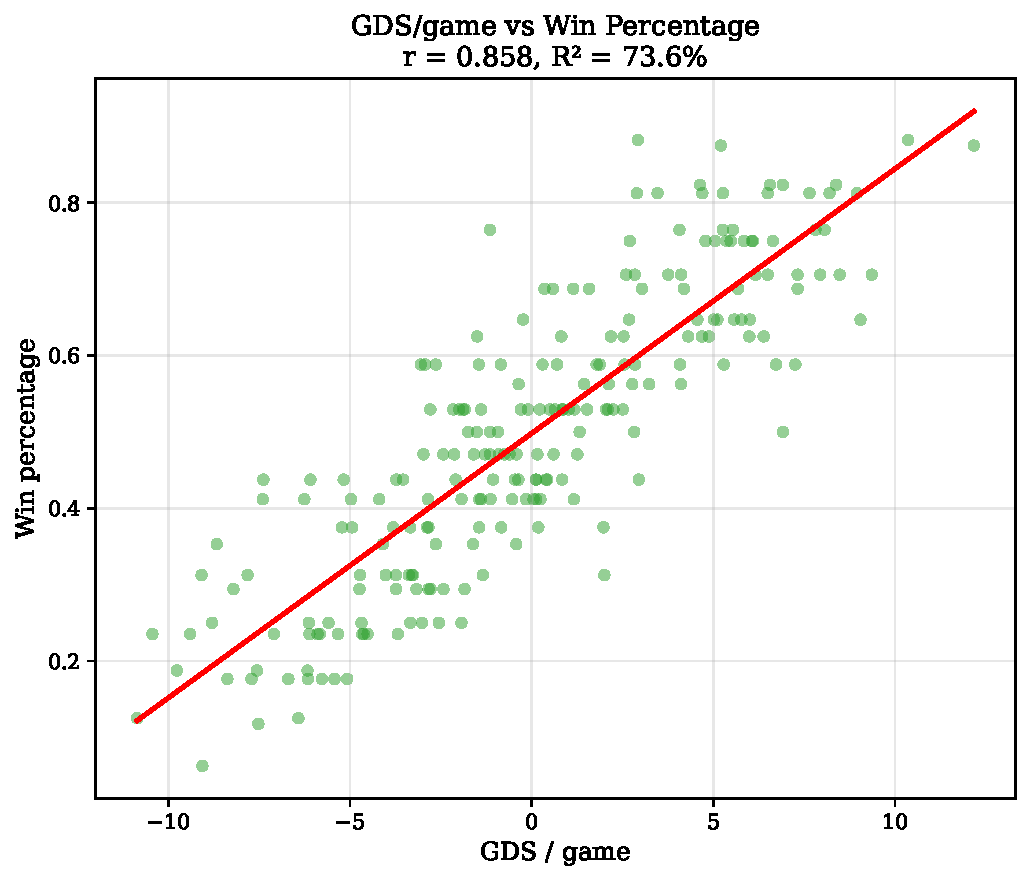
\includegraphics[width=0.7\textwidth]{figures/fig6_gds_vs_winpct.pdf}
  \caption{Season-level GDS/game versus win percentage ($N = 224$
           team-seasons, 2018--2024). The tight linear relationship
           ($r = 0.858$, $R^2 = 73.6\%$) confirms that GDS captures
           the underlying competitive quality dimension that drives
           winning.}
  \label{fig:gds-winpct}
\end{figure}

\subsubsection*{Component Decomposition of Explained Variance}

The three-component structure of \gds{} permits a direct comparison of the
individual explanatory contributions of offense and defense. \Cref{tab:component-variance}
presents the correlation and $R^2$ for each component in isolation alongside
the combined \gds{}.

\begin{table}[htbp]
  \centering
  \caption{Correlation between individual \gds{} components and season win
           percentage ($n = 224$ team-seasons, 2018--2024). The combined
           \gds{}/game value exceeds the sum of individual $R^2$ contributions,
           confirming that the components carry partially non-overlapping
           information about team success.}
  \label{tab:component-variance}
  \begin{tabular}{lccc}
    \toprule
    \textbf{Metric} & \textbf{Pearson $r$} & \textbf{95\% CI} & \textbf{$R^2$} \\
    \midrule
    Offensive \xvoa{}/game  & 0.681 & [0.608, 0.743] & 0.464 \\
    Defensive \xvoa{}/game  & 0.376 & [0.260, 0.483] & 0.142 \\
    Combined \gds{}/game    & 0.858 & [0.824, 0.888] & 0.736 \\
    \bottomrule
  \end{tabular}
\end{table}

Several findings follow from this decomposition. First, offensive \xvoa{} is
the dominant predictor of season-level success, explaining 46.4\% of win-rate
variance individually. This is consistent with the broader NFL analytics
literature, which finds that passing efficiency and drive conversion are the
primary drivers of team-level outcomes \parencite{yurko2019nflwar}. Second,
defensive \xvoa{} adds a distinct and meaningful explanatory channel, accounting
for 14.2\% of variance individually. Third, the combined \gds{} $R^2$ of 0.736
substantially exceeds the sum of individual $R^2$ values (46.4\% + 14.2\% =
60.6\%), a 13.0 percentage point surplus indicating that the whole is greater
than the sum of its parts. The combined metric captures interaction effects
between offensive and defensive quality -- teams that are strong on both
dimensions outperform the additive expectation more than a pure linear model
of each component would predict. This synergistic structure justifies treating
\gds{} as a unified team-quality index rather than as a simple sum of
independent components \parencite{robst2011defense}.

\Cref{fig:xvoa-winpct} visualizes this asymmetry: the offensive scatter is
markedly tighter than the defensive scatter, reflecting the $3.3 : 1$ ratio in
explained variance.

\begin{figure}[htbp]
  \centering
  
\includegraphics[width=\textwidth]{figures/fig3_xvoa_vs_winpct.pdf}
  \caption{Offensive (left) and defensive (right) xVOA/game vs.\ win
           percentage. The tighter clustering and steeper regression line for
           offense visually demonstrate that offensive quality explains
           substantially more win-rate variance ($R^2 = 46.4\%$) than
           defensive quality ($R^2 = 14.2\%$).}
  \label{fig:xvoa-winpct}
\end{figure}

%  -- -- -- -- -- -- -- -- -- -- -- -- -- -- -- -- -- -- -- --
\subsection{Component Structure of Top and Bottom Teams}
\label{sec:component-decomposition}

The season-level correlation analysis demonstrates that \gds{} is a valid
aggregate predictor. The component decomposition of individual team-seasons
reveals the structural diversity that the framework captures: there is more
than one path to a high \gds{}, and the winning formulas of top teams differ
substantially in their offensive and defensive balance.

\Cref{tab:gds-top-bottom} presents the five highest and five lowest \gds{}/game
teams in the 2024 NFL regular season, with component breakdowns for offensive
and defensive \xvoa{}.

\begin{table}[htbp]
  \centering
  \caption{Top-5 and bottom-5 NFL teams by \gds{}/game in the 2024 regular
           season, with component breakdown. Offensive and defensive \xvoa{}
           are reported per game. Win\% is the regular-season win proportion.
           Teams are sorted by descending \gds{}/game within each panel.}
  \label{tab:gds-top-bottom}
  \begin{tabular}{lrrrr}
    \toprule
    \textbf{Team} & \textbf{\gds{}/G} & \textbf{Off \xvoa{}/G}
      & \textbf{Def \xvoa{}/G} & \textbf{Win\%} \\
    \midrule
    \multicolumn{5}{l}{\textit{Top 5}} \\[2pt]
    DET & $+10.365$ & $+12.980$ & $-2.630$ & 0.882 \\
    PHI & $+8.384$  & $+7.740$  & $+0.639$ & 0.824 \\
    BAL & $+7.945$  & $+11.035$ & $-3.068$ & 0.706 \\
    TB  & $+6.729$  & $+10.586$ & $-3.822$ & 0.588 \\
    GB  & $+5.575$  & $+6.462$  & $-0.999$ & 0.647 \\[6pt]
    \multicolumn{5}{l}{\textit{Bottom 5}} \\[2pt]
    JAX & $-5.835$  & $+1.306$  & $-7.158$  & 0.235 \\
    NYG & $-6.158$  & $-2.417$  & $-3.799$  & 0.176 \\
    DAL & $-6.259$  & $+0.745$  & $-7.002$  & 0.412 \\
    CLE & $-6.700$  & $-5.861$  & $-1.012$  & 0.176 \\
    CAR & $-8.211$  & $+2.616$  & $-10.852$ & 0.294 \\
    \bottomrule
  \end{tabular}
\end{table}

Four structural observations emerge from this table.

\paragraph{Offense dominates the top.}
The five highest-\gds{} teams in 2024 all derive the majority of their
\gds{} from offense. Detroit (DET) is the most extreme case: their offensive
\xvoa{} of $+12.980$/game is the largest in the sample, paired with a
\emph{negative} defensive contribution ($-2.630$). Baltimore (BAL) follows a
similar structure -- a dominant offense ($+11.035$) paired with below-average
defense ($-3.068$). The Eagles (PHI) are the only top-five team with a
positive defensive \xvoa{} ($+0.639$), making them the most balanced elite
profile in 2024. Tampa Bay (TB) presents a striking case: elite offense
($+10.586$) paired with the worst defense among the top five ($-3.822$), yet
still the fourth-best overall \gds{}.

\paragraph{The role of defense: at best a complement.}
Among the top five teams, four record negative defensive \xvoa{} -- their
defenses performed \emph{below league-average expectations} at the drive level.
This observation reinforces the finding from \Cref{sec:season-correlation}:
it is entirely possible to be a top-tier team while running a below-average
defense, provided the offensive surplus is sufficiently large. Philadelphia's
modest positive defensive contribution ($+0.639$) shows that defensive
excellence can augment offensive quality, but it is not the primary engine
of overall \gds{} for any top-five team.

\paragraph{Defense drives the floor.}
The five lowest-\gds{} teams display a different structural pattern.
While Cleveland (CLE) fits the expected archetype of offensive collapse
($-5.861$/game), three of the five bottom teams -- Jacksonville (JAX),
Dallas (DAL), and Carolina (CAR) -- actually record \emph{positive}
offensive \xvoa{}. Their bottom-tier status is driven almost entirely by
catastrophic defensive performance: Carolina's defensive \xvoa{} of
$-10.852$/game is the most extreme defensive deficit in the 2024 sample.
This finding reveals that while offensive quality is the primary
\emph{predictor} of success, extreme defensive failure can override even
positive offensive production.

\paragraph{Asymmetric variance across phases.}
The range of offensive \xvoa{}/game in 2024 spans from $-5.861$ (CLE) to
$+12.980$ (DET), a spread of 18.8 points. The defensive range spans from
$-10.852$ (CAR) to $+0.639$ (PHI), a spread of 11.5 points but skewed
heavily negative -- most teams record negative defensive \xvoa{}, consistent
with the higher baseline variance in offensive execution.

%  -- -- -- -- -- -- -- -- -- -- -- -- -- -- -- -- -- -- -- --
\subsection{Luck Analysis: GDS-Implied vs Actual Wins}
\label{sec:luck-analysis}

Even a validated team-quality metric should not be expected to perfectly predict
win totals, because NFL games contain structural sources of variance that are
not reflected in the underlying execution quality measured by \gds{}: fumble
recovery rates, turnover-for-touchdown conversion, the resolution of close
games decided by a single late possession, and kick special teams variance.
The gap between a team's \gds{}-implied expected wins and their actual win total
is a natural operationalization of \emph{luck}: teams with large positive
divergences (more wins than expected) benefited from variance; teams with
large negative divergences (fewer wins than expected) were penalized by it.

\Cref{tab:luck-analysis} reports the most extreme cases in the 2024 season.
Expected wins are derived by applying the cross-season regression relationship
between \gds{}/game and win rate to each team's observed \gds{}/game value;
the implied win count is then obtained by scaling by 17 games. This linear
extrapolation can produce implied win totals outside the feasible range
(0--17) for extreme \gds{} values; such cases should be interpreted as
indicating floor or ceiling effects rather than literal win predictions.

\begin{table}[htbp]
  \centering
  \caption{Luckiest and unluckiest teams in the 2024 NFL regular season by
           the divergence between actual wins and \gds{}-implied wins.
           Positive divergence (luckiest) indicates more actual wins than
           the team's execution quality warranted; negative divergence
           (unluckiest) indicates fewer wins than expected.}
  \label{tab:luck-analysis}
  \begin{tabular}{lrrr}
    \toprule
    \textbf{Team} & \textbf{Actual Wins} & \textbf{GDS-Implied Wins}
      & \textbf{Divergence} \\
    \midrule
    \multicolumn{4}{l}{\textit{Luckiest}} \\[2pt]
    KC  & 15 & ${\approx}10.2$ & $+4.8$ \\
    HOU & 10 & ${\approx}6.7$  & $+3.3$ \\
    LA  & 10 & ${\approx}6.9$  & $+3.1$ \\[6pt]
    \multicolumn{4}{l}{\textit{Unluckiest}} \\[2pt]
    TEN &  3 & ${\approx}5.5$  & $-2.5$ \\
    TB  & 10 & ${\approx}12.4$ & $-2.4$ \\
    NYJ &  5 & ${\approx}7.0$  & $-2.0$ \\
    \bottomrule
  \end{tabular}
\end{table}

The Kansas City (KC) case is the most striking. With a moderate \gds{}/game of
$+2.92$, the regression model implies approximately 10.2 wins; yet Kansas City
finished with 15 wins, the largest positive divergence ($+4.8$) in 2024. This
surplus represents a team that consistently converted close-game situations in
their favor -- a pattern consistent with Kansas City's well-documented
fourth-quarter performance under Patrick Mahomes and Andy Reid. Houston (HOU)
and the Rams (LA) similarly outperformed their \gds{}-implied win totals by
approximately 3 wins each, representing teams with below-average execution
quality that benefited from favorable variance in game outcomes.

At the other end of the divergence distribution, Tampa Bay (TB) was the most
conspicuously unlucky team of 2024. With the fourth-highest \gds{} in the
league ($+6.729$/game), they finished with only 10 wins against an implied
expectation of roughly 12.4. Tennessee (TEN) experienced a similar negative
divergence ($-2.5$), winning only 3 games despite execution quality
implying approximately 5.5 wins.

The New York Jets (NYJ) present a further instructive case: a team with an
implied expectation of roughly 7 wins that finished with only 5, suggesting
that their 2024 record overstates their competitive weakness relative to the
underlying process.

The existence of these systematic divergences between deserved and actual
outcomes reinforces the core motivation for the \gds{} framework: win-loss
records are an imperfect proxy for team quality, and a measure of
\emph{process} rather than \emph{outcome} provides additional information
for evaluating past performance and projecting future competitiveness.

%  -- -- -- -- -- -- -- -- -- -- -- -- -- -- -- -- -- -- -- --
\subsection{Summary}
\label{sec:gds-validation-summary}

Four lines of evidence collectively validate the \gds{} framework as a
meaningful measure of team-level competitive quality. Game-level winner
prediction achieves 86.1\% accuracy across 1{,}848 regular-season contests,
compared to a na\"{i}ve home-team baseline of 57\% -- a gap of 29 percentage
points that confirms \gds{} tracks the underlying performance process rather
than the noise of individual outcomes. At the season level, \gds{}/game
explains 73.6\% of win-percentage variance ($r = 0.858$, $p = 3.24 \times 10^{-66}$,
$n = 224$ team-seasons), with offense contributing 46.4\% and defense 14.2\%
individually and the combined metric exceeding both. The 2024 component
decomposition reveals the structural diversity of competitive profiles at the
top of the distribution -- offense-dominant, defense-dominant, and balanced
configurations all achieve high \gds{} -- while confirming that the bottom of
the distribution is consistently defined by offensive failure. The luck
analysis demonstrates that win-loss records carry substantial noise relative
to the underlying execution signal, with team divergences as large as $\pm 3$--5
wins in a single season.

Having established that \gds{} is a validated measure of deserved competitive
performance, the archetype analysis in \Cref{sec:archetype-findings} proceeds
from the premise that \gds{} component profiles constitute a meaningful basis
for classifying teams by strategic identity.
